\documentclass{standalone}
\usepackage{tikz}
\usetikzlibrary{patterns}
\usetikzlibrary{positioning}
\usetikzlibrary{patterns, positioning}
\usetikzlibrary{shapes.misc}
\usepackage[outline]{contour}
\contourlength{1.5pt} 
\usepackage[sfdefault]{ClearSans}

\begin{document}
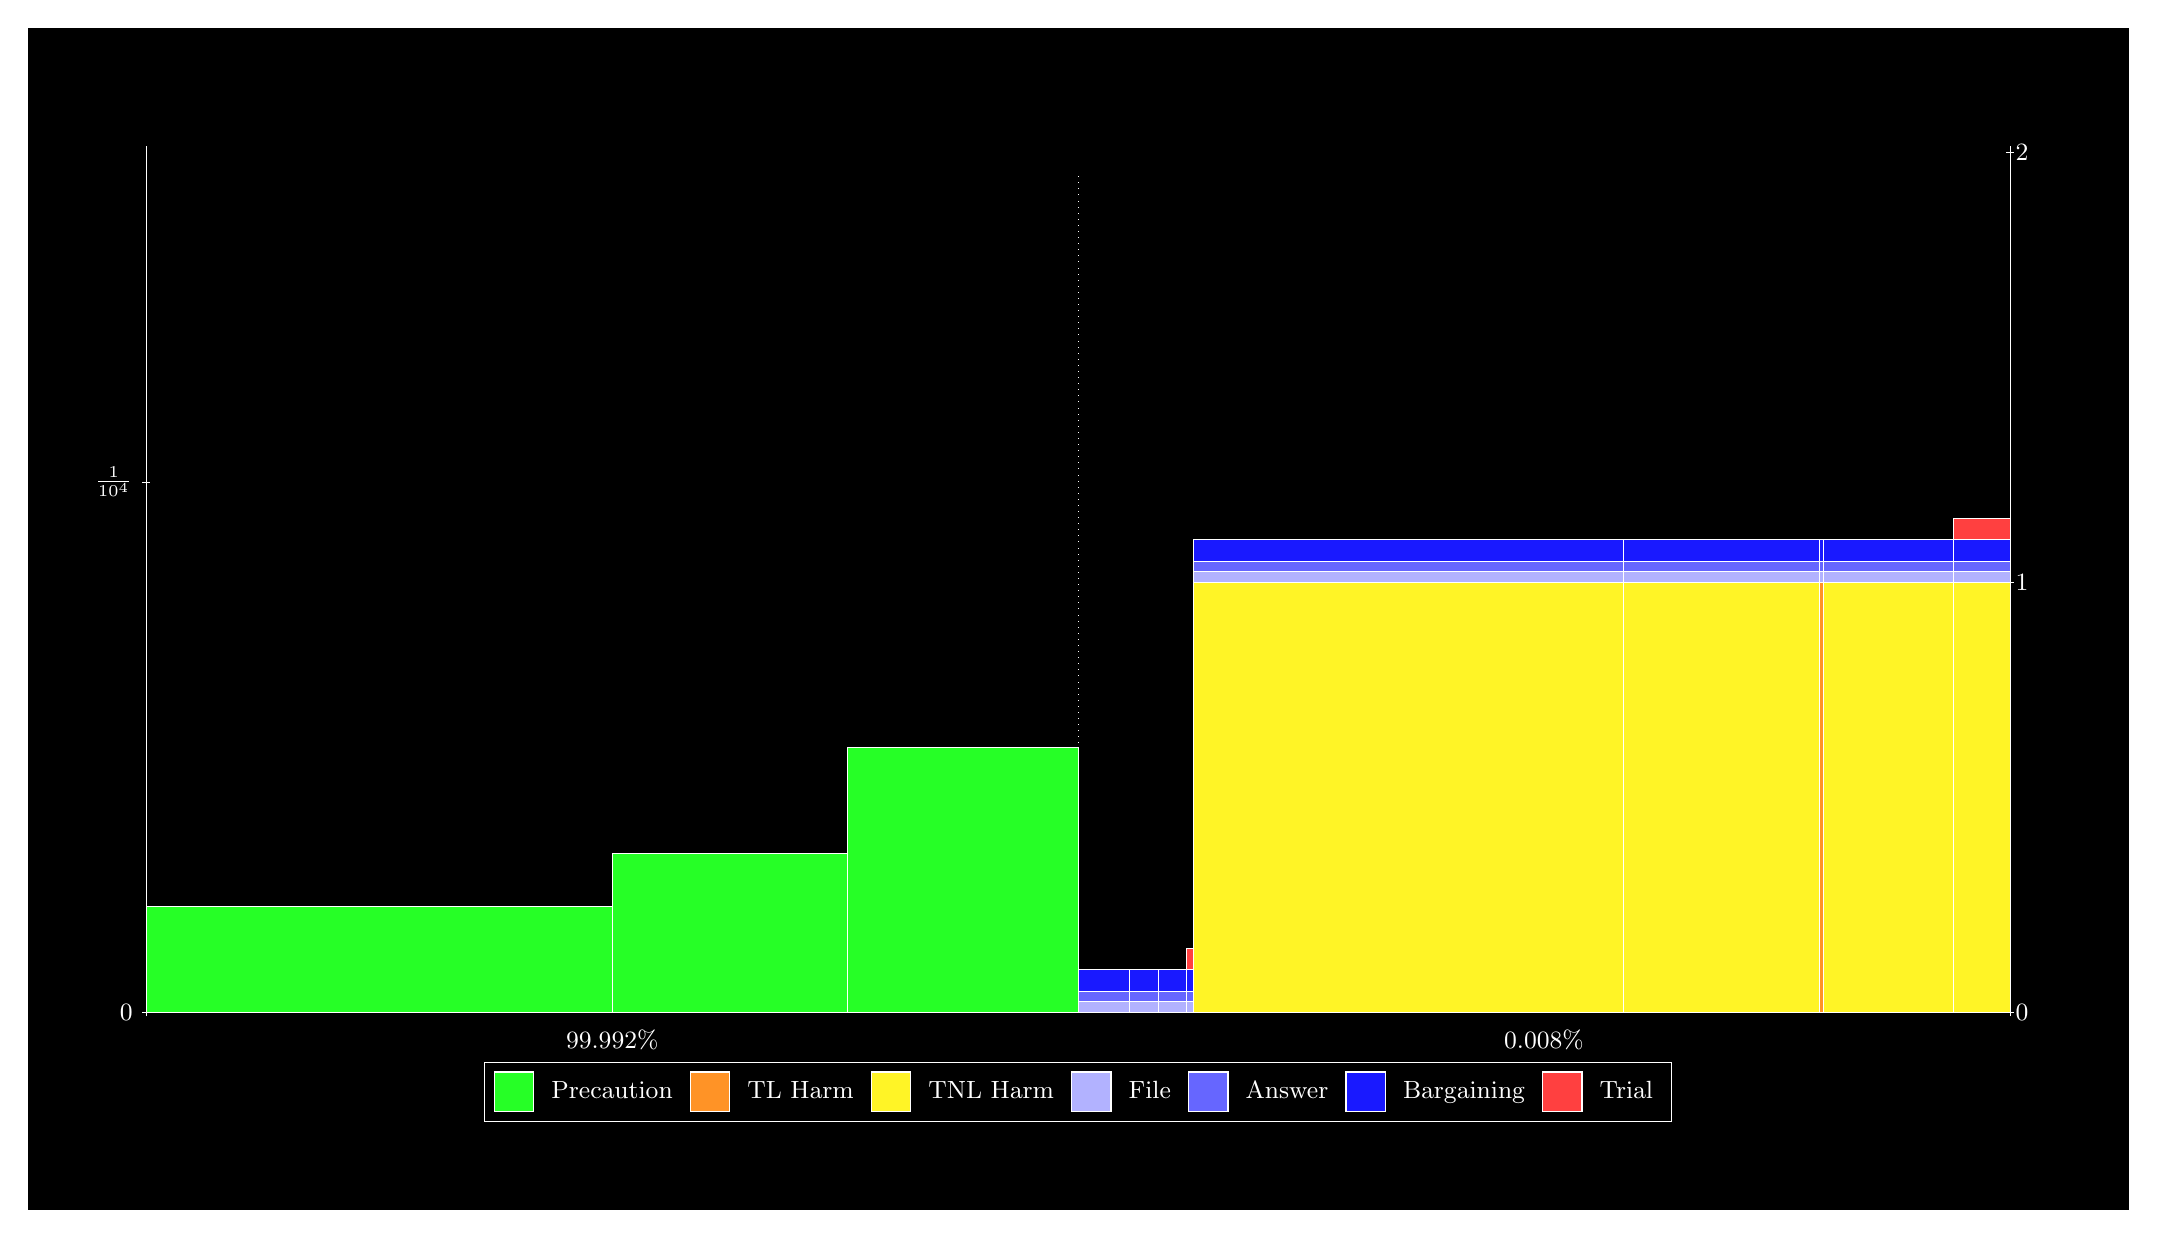
\begin{tikzpicture}
\draw[fill=black] (0,0) rectangle (26.667,15);
\draw[fill=green!85,draw=white,very thin] (1.5,2.5) rectangle (7.4166,3.8478);
\draw[fill=green!85,draw=white,very thin] (7.4166,2.5) rectangle (10.403,4.5217);
\draw[fill=green!85,draw=white,very thin] (10.403,2.5) rectangle (13.333,5.8695);
\draw[fill=green!85,draw=white,very thin] (13.333,2.5) rectangle (13.978,2.5001);
\draw[fill=blue!30,draw=white,very thin] (13.333,2.5001) rectangle (13.978,2.6367);
\draw[fill=blue!60,draw=white,very thin] (13.333,2.6367) rectangle (13.978,2.7732);
\draw[fill=blue!90,draw=white,very thin] (13.333,2.7732) rectangle (13.978,3.0463);
\draw[fill=green!85,draw=white,very thin] (13.978,2.5) rectangle (14.347,2.5002);
\draw[fill=blue!30,draw=white,very thin] (13.978,2.5002) rectangle (14.347,2.6367);
\draw[fill=blue!60,draw=white,very thin] (13.978,2.6367) rectangle (14.347,2.7733);
\draw[fill=blue!90,draw=white,very thin] (13.978,2.7733) rectangle (14.347,3.0464);
\draw[fill=green!85,draw=white,very thin] (14.347,2.5) rectangle (14.71,2.5003);
\draw[fill=blue!30,draw=white,very thin] (14.347,2.5003) rectangle (14.71,2.6368);
\draw[fill=blue!60,draw=white,very thin] (14.347,2.6368) rectangle (14.71,2.7734);
\draw[fill=blue!90,draw=white,very thin] (14.347,2.7734) rectangle (14.71,3.0465);
\draw[fill=green!85,draw=white,very thin] (14.71,2.5) rectangle (14.795,2.5001);
\draw[fill=blue!30,draw=white,very thin] (14.71,2.5001) rectangle (14.795,2.6367);
\draw[fill=blue!60,draw=white,very thin] (14.71,2.6367) rectangle (14.795,2.7732);
\draw[fill=blue!90,draw=white,very thin] (14.71,2.7732) rectangle (14.795,3.0463);
\draw[fill=red!75,draw=white,very thin] (14.71,3.0463) rectangle (14.795,3.3194);
\draw[fill=green!85,draw=white,very thin] (14.795,2.5) rectangle (20.256,2.5001);
\draw[fill=yellow!85,draw=white,very thin] (14.795,2.5001) rectangle (20.256,7.962);
\draw[fill=blue!30,draw=white,very thin] (14.795,7.962) rectangle (20.256,8.0986);
\draw[fill=blue!60,draw=white,very thin] (14.795,8.0986) rectangle (20.256,8.2351);
\draw[fill=blue!90,draw=white,very thin] (14.795,8.2351) rectangle (20.256,8.5082);
\draw[fill=green!85,draw=white,very thin] (20.256,2.5) rectangle (22.752,2.5002);
\draw[fill=yellow!85,draw=white,very thin] (20.256,2.5002) rectangle (22.752,7.9621);
\draw[fill=blue!30,draw=white,very thin] (20.256,7.9621) rectangle (22.752,8.0986);
\draw[fill=blue!60,draw=white,very thin] (20.256,8.0986) rectangle (22.752,8.2352);
\draw[fill=blue!90,draw=white,very thin] (20.256,8.2352) rectangle (22.752,8.5083);
\draw[fill=green!85,draw=white,very thin] (22.752,2.5) rectangle (22.796,2.5002);
\draw[fill=orange!85,draw=white,very thin] (22.752,2.5002) rectangle (22.796,7.9621);
\draw[fill=blue!30,draw=white,very thin] (22.752,7.9621) rectangle (22.796,8.0986);
\draw[fill=blue!60,draw=white,very thin] (22.752,8.0986) rectangle (22.796,8.2352);
\draw[fill=blue!90,draw=white,very thin] (22.752,8.2352) rectangle (22.796,8.5083);
\draw[fill=green!85,draw=white,very thin] (22.796,2.5) rectangle (24.446,2.5003);
\draw[fill=yellow!85,draw=white,very thin] (22.796,2.5003) rectangle (24.446,7.9622);
\draw[fill=blue!30,draw=white,very thin] (22.796,7.9622) rectangle (24.446,8.0987);
\draw[fill=blue!60,draw=white,very thin] (22.796,8.0987) rectangle (24.446,8.2353);
\draw[fill=blue!90,draw=white,very thin] (22.796,8.2353) rectangle (24.446,8.5084);
\draw[fill=green!85,draw=white,very thin] (24.446,2.5) rectangle (25.167,2.5001);
\draw[fill=yellow!85,draw=white,very thin] (24.446,2.5001) rectangle (25.167,7.962);
\draw[fill=blue!30,draw=white,very thin] (24.446,7.962) rectangle (25.167,8.0986);
\draw[fill=blue!60,draw=white,very thin] (24.446,8.0986) rectangle (25.167,8.2351);
\draw[fill=blue!90,draw=white,very thin] (24.446,8.2351) rectangle (25.167,8.5082);
\draw[fill=red!75,draw=white,very thin] (24.446,8.5082) rectangle (25.167,8.7813);
\draw[white,very thin] (1.5,2.5) -- (1.5,13.5);
\draw[white,very thin] (1.45,2.5) -- (1.55,2.5);
\node[font=\small,text=white, anchor=east] at (1.45, 2.5) {0};
\draw[white,very thin] (1.45,9.2389) -- (1.55,9.2389);
\node[font=\small,text=white, anchor=east] at (1.45, 9.2389) {$\frac{1}{10^{4}}$};

\draw[white,dotted,very thin] (13.333,2.83) -- (13.333,13.17);
\draw[white,very thin] (25.167,2.5) -- (25.167,13.5);
\draw[white,very thin] (25.117,2.5) -- (25.217,2.5);
\node[font=\small,text=white, anchor=west] at (25.117, 2.5) {0};
\draw[white,very thin] (25.117,7.9619) -- (25.217,7.9619);
\node[font=\small,text=white, anchor=west] at (25.117, 7.9619) {1};
\draw[white,very thin] (25.117,13.424) -- (25.217,13.424);
\node[font=\small,text=white, anchor=west] at (25.117, 13.424) {2};

\draw[white,very thin] (1.5,2.5) -- (25.167,2.5);
\draw[white,very thin] (1.5,2.45) -- (1.5,2.55);
\node[font=\small,text=white, anchor=north] at (1.5, 2.45) {};
\draw[white,very thin] (25.167,2.45) -- (25.167,2.55);
\node[font=\small,text=white, anchor=north] at (25.167, 2.45) {};

\node[font=\small,text=white,anchor=south] at (7.4167, 1.9) {99.992\%};
\node[font=\small,text=white,anchor=south] at (19.25, 1.9) {0.008\%};
\draw (13.3333,2.5) node (B) {};
\begin{scope}[align=center]
\matrix[scale=0.5,draw=white,below=0.5cm of B,nodes={draw},column sep=0.1cm]{
\node[rectangle,draw,minimum width=0.5cm,minimum height=0.5cm,fill=green!85]{}; & \node[draw=none,font=\small,text=white]{Precaution}; &
\node[rectangle,draw,minimum width=0.5cm,minimum height=0.5cm,fill=orange!85]{}; & \node[draw=none,font=\small,text=white]{TL Harm}; &
\node[rectangle,draw,minimum width=0.5cm,minimum height=0.5cm,fill=yellow!85]{}; & \node[draw=none,font=\small,text=white]{TNL Harm}; &
\node[rectangle,draw,minimum width=0.5cm,minimum height=0.5cm,fill=blue!30]{}; & \node[draw=none,font=\small,text=white]{File}; &
\node[rectangle,draw,minimum width=0.5cm,minimum height=0.5cm,fill=blue!60]{}; & \node[draw=none,font=\small,text=white]{Answer}; &
\node[rectangle,draw,minimum width=0.5cm,minimum height=0.5cm,fill=blue!90]{}; & \node[draw=none,font=\small,text=white]{Bargaining}; &
\node[rectangle,draw,minimum width=0.5cm,minimum height=0.5cm,fill=red!75]{}; & \node[draw=none,font=\small,text=white]{Trial}; \\\\
};\end{scope}

\end{tikzpicture}
\end{document}